\documentclass[a4paper,twoside]{article}
\usepackage{blindtext}  
\usepackage{geometry}

% Chinese support
\usepackage[UTF8, scheme = plain]{ctex}

% Page margin layout
\geometry{left=2.3cm,right=2cm,top=2.5cm,bottom=2.0cm}


\usepackage{listings}
\usepackage{xcolor}
\usepackage{geometry}
\usepackage{amsmath}
\usepackage{float}
\usepackage{hyperref}

\usepackage{graphics}
\usepackage{graphicx}
\usepackage{subcaption}
\usepackage{epsfig}
\usepackage{float}

\usepackage{algorithm}
\usepackage[noend]{algpseudocode}

\usepackage{booktabs}
\usepackage{threeparttable}
\usepackage{longtable}
\usepackage{tikz}
\usepackage{multicol}

% cite package, to clean up citations in the main text. Do not remove.
\usepackage{cite}

\usepackage{color,xcolor}

%% The amssymb package provides various useful mathematical symbols
\usepackage{amssymb}
%% The amsthm package provides extended theorem environments
\usepackage{amsthm}
\usepackage{amsfonts}
\usepackage{enumerate}
\usepackage{enumitem}
\usepackage{listings}
\usepackage{minted}


\usepackage{indentfirst}
\setlength{\parindent}{2em} % Make two letter space in the first paragraph
\usepackage{setspace}
\linespread{1.5} % Line spacing setting
\usepackage{siunitx}
\setlength{\parskip}{0.5em} % Paragraph spacing setting

% \usepackage[contents =22920202204622, scale = 10, color = black, angle = 50, opacity = .10]{background}

\renewcommand{\figurename}{图}
\renewcommand{\listingscaption}{代码}
\renewcommand{\tablename}{表格}
\renewcommand{\contentsname}{目录}
\floatname{algorithm}{算法}

\graphicspath{ {images/} }

%%%%%%%%%%%%%
\newcommand{\StudentNumber}{22920202204622}  % Fill your student number here
\newcommand{\StudentName}{熊恪峥}  % Replace your name here
\newcommand{\PaperTitle}{实验(四)用Yacc实现语法分析器}  % Change your paper title here
\newcommand{\PaperType}{编译原理} % Replace the type of your report here
\newcommand{\Date}{2023年5月20日}
\newcommand{\College}{信息学院}
\newcommand{\CourseName}{编译原理}
%%%%%%%%%%%%%

%% Page header and footer setting
\usepackage{fancyhdr}
\usepackage{lastpage}
\pagestyle{fancy}
\fancyhf{}
% This requires the document to be twoside
\fancyhead[LO]{\texttt{\StudentName }}
\fancyhead[LE]{\texttt{\StudentNumber}}
\fancyhead[C]{\texttt{\PaperTitle }}
\fancyhead[R]{\texttt{第{\thepage}页,共\pageref*{LastPage}页}}


\title{\PaperTitle}
\author{\StudentName}
\date{\Date}

\algnewcommand\algorithmicinput{\textbf{Input:}}
\algnewcommand\algorithmicoutput{\textbf{Output:}}
\algnewcommand\Input{\item[\algorithmicinput]}%
\algnewcommand\Output{\item[\algorithmicoutput]}%

\newenvironment{longlisting}{\captionsetup{type=figure}}{}

\usetikzlibrary{positioning, shapes.geometric}

\begin{document}
	
%%%%%%%%%%%%%%%%%%%%%%%%%%%%%%%%%%%%%%%%%%%%
\makeatletter % change default title style
\renewcommand*\maketitle{%
	\begin{center} 
		\bfseries  % title 
		{\LARGE \@title \par}  % LARGE typesetting
		\vskip 1em  %  margin 1em
		{\global\let\author\@empty}  % no author information
		{\global\let\date\@empty}  % no date
		\thispagestyle{empty}   %  empty page style
	\end{center}%
	\setcounter{footnote}{0}%
}
\makeatother
%%%%%%%%%%%%%%%%%%%%%%%%%%%%%%%%%%%%%%%%%%%%
	
	
\thispagestyle{empty}

\vspace*{1cm}

\begin{figure}[htb]
	\centering
	
\includegraphics[width=4.0cm]{logo.png}
\end{figure}

\vspace*{1cm}

\begin{center}
	\Huge{\textbf{\PaperType}}
	
	\Large{\PaperTitle}
\end{center}

\vspace*{1cm}

\begin{table}[H]
	\centering	
	\begin{Large}
		\renewcommand{\arraystretch}{1.5}
		\begin{tabular}{p{3cm} p{5cm}<{\centering}}
			姓\qquad 名 & \StudentName  \\
			\hline
			学\qquad号 & \StudentNumber \\
			\hline
			日\qquad期 & \Date  \\
			\hline
			学\qquad院 & \College  \\
			\hline
			课程名称 & \CourseName  \\
			\hline
		\end{tabular}
	\end{Large}
\end{table}

\newpage

\title{
	\Large{\textcolor{black}{\PaperTitle}}
}
	
	
\maketitle
	
\tableofcontents
 
\newpage
\setcounter{page}{1}

\begin{spacing}{1.2}

\section{实验目的}

掌握语法分析器的构造原理,掌握Yacc的编程方法。

\section{实验内容}

用Yacc编写一个语法分析程序,使之与词法分析器结合,能够根据语言的上下文无关文法,识别输入的单词序列是否文法的句子。

\section{运行结果}

运行结果如图~\ref{fig:output},完整输出见\nameref{sec:fullout}。
\begin{figure}[htb]
	\centering
	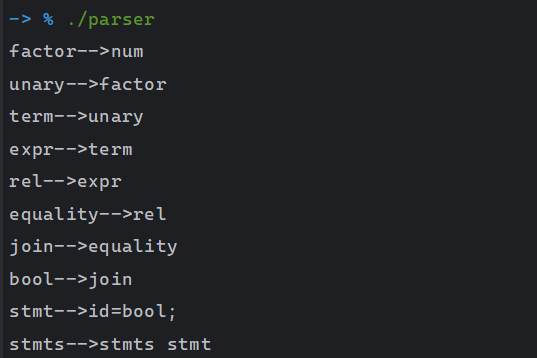
\includegraphics[width=0.6\linewidth]{output.png}
	\caption{运行结果}
	\label{fig:output}
\end{figure}

\section{支持前缀'-'和'!'运算符}

在这次实验中,我额外实现了对前缀'-'和'!'运算符的支持,即取相反数运算符和逻辑非运算符。

首先,需要对文法进行改写。该文法的优先级应该高于乘除法,但低于加减法。据此编写处理一元运算符的文法如下:
\inputminted{c}{text/grammar.txt}

同时,对于前缀'-'运算符需要处理结合性。
在上述文法中通过标记\texttt{UMINUS}指定了\texttt{\%nonassoc},
意为无结合性。这样,yacc会将形如\texttt{a op b op c}式的表达式视为错误。
这样做的目的在于区分二元'-'运算符,即减法运算符。
通过指定无结合性,二元'-'运算符和一元'-'运算符得以区分,不会产生冲突的问题。
否则,yacc就会输出产生移入规约冲突的信息。

\appendix
\section{附录:完整输出}
\label{sec:fullout}

\inputminted{bnf}{text/output.txt}

\end{spacing}

\end{document}